\section{Authorization in Client-Server Application}
\paragraph{HTTP is stateless} so any request must "recall" who it is. But many services are \textbf{session oriented} meaning it stores state information for the session. Here we will see several ways to authenticate the user.

\subsection{Session Cookies}
\paragraph{Main idea} is during login, the server generates a session token and sends it to the client as a cookie which is stored inside the browser and associated with the domain then re-used in every query to that website. See Figure \ref{fig:token}

\begin{figure}
    \centering
    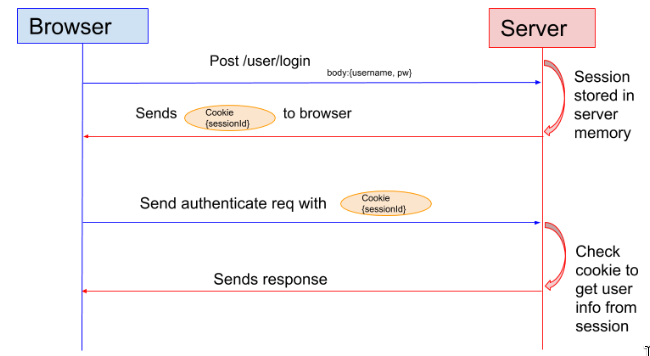
\includegraphics[width = 0.7 \linewidth]{Figures/Token.png}
    \caption{Session Token}
    \label{fig:token}
\end{figure}

This allows a potential attacker to hijack the session by using the same cookie to send requests to the web server and prentend to be the user.

\paragraph{Securing the Session token} is possible with different techniques such as Same-origin policy mentioned before as well as using (ofc) HTTPS to protect the traffic between user and web server. It is also important to make the session token as \textbf{unpredictable} as possiblee

\textbf{Advantage} : is that a token can easily be revoked by removing it from the server's internal state

\textbf{Disadvantage} : is that sever needs to store a hash table and access it at every request which is inneficient.

\subsection{JSON Web Tokens}
\paragraph{What} A JWT is a essentially a signed token issued by a server and stored by the client. 

\paragraph{How}  It contains a set of claims (e.g., user ID, role, session ID, expiration time) together with a server-generated signature. The client includes the JWT in further requests (e.g., in a cookie or HTTP header). 

\paragraph{Why}The signature allows the server to verify that the token has not been modified by the client. JWTs can be used in both stateful and stateless session architectures. Since JWTs are typically only Base64-encoded and not encrypted, their contents should not be considered secret; confidentiality is usually provided by TLS during transmission.

\subsection{OAuth}
\paragraph{Motivation} Traditional user/pwd protection is limited as for third party app to use a service under your name it would require it to know your password and if you were not to want that third party to use a service you would need to change your pswd... 

\paragraph{Main idea} instead of giving an app a password, you give it a temporary permission token.

Here is the complete flow (see Figure \ref{fig:OAuth})

\begin{figure}
    \centering
    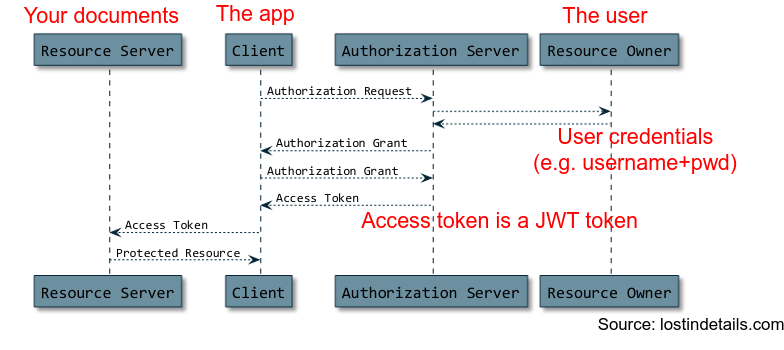
\includegraphics[width = 0.7 \linewidth]{Figures/OAuth.png}
    \caption{OAuth Flow}
    \label{fig:OAuth}
\end{figure}

Here are the different steps:
\begin{itemize} 
    \item \textbf{Authorization Request}: The client (e.g. ILovePDF) sends a request to the Authorization Server of the resource owner (e.g. Dropbox). The request contains a \textbf{scope} describing the permissions being requested (e.g. read, write) and a \textbf{client identifier} that identifies the application. The resource owner can then approve or deny the requested permissions. 
    
    \item \textbf{Authorization Grant}: If the resource owner approves the request, the Authorization Server sends an \textbf{authorization code} back to the client. This code is short-lived and can only be used \textbf{once}. It is not an access token yet. 
    
    \item \textbf{Token Request}: The client sends the authorization code back to the Authorization Server to exchange it for an \textbf{access token}. This request also contains information proving the identity of the client, such as a \textbf{client secret} or a PKCE verifier. 
    
    \item \textbf{Access Token}: The Authorization Server verifies the code and the client identity. If everything is valid, it returns an access token. The client can then use this token to access the protected resources.
    
    \item \textbf{Resource Access}: The client sends the access token to the Resource Server when requesting protected data. The Resource Server accepts the request only if the token is valid and has the required scope. 
    
    \item \textbf{Refresh Token}: Since access tokens are usually short-lived, the Authorization Server may also issue a refresh token. The client can use it to obtain a new access token without repeating the full authorization code flow. 
    
    \item \textbf{Token Verification}: The Resource Server must verify that an access token is valid. This can be done locally if the token is a signed JWT, or by asking the Authorization Server using token introspection. 

\end{itemize} 


\paragraph{Why not directly return the access token?} OAuth2 could directly return the access token to the client. This is called the \textbf{Implicit Flow}. However, this is generally not recommended because the access token is directly usable to access resources. If it is exposed in a browser redirect, URL, log, or history, an attacker can immediately use it. The Authorization Code Flow is safer because the first redirect only contains an authorization code: \[ \texttt{code=XYZABC} \] This code is not directly usable to access resources. It must first be exchanged for an access token. During this exchange, the Authorization Server can verify the client again using a client secret or PKCE. 


\paragraph{Important distinction} 
\begin{itemize} 
    \item \textbf{Client ID}: public identifier of the application. 
    \item \textbf{Client secret / PKCE verifier}: proves that the client is legitimate.
    
    \item \textbf{Authorization code}: short-lived, one-time proof that the user approved access. 
    
    \item \textbf{Access token}: actual credential used to access protected resources. 

\end{itemize}

If an attacker steals an access token, they can usually use it until it expires. Therefore, access tokens should be protected with HTTPS, stored securely, and given short lifetimes. 

\paragraph{Remarks} OAuth2 is an \textbf{authorization framework}, not an authentication protocol. It defines how a client application obtains permission to access resources, but it does not define how the user is authenticated. Authentication can be added on top of OAuth2 using protocols such as OpenID Connect. 

OAuth2 is difficult to implement correctly, so existing libraries should be used whenever possible.